\section{Aggressive Prunability and Symbolic Distillation}
\label{sec:pruning}

A key empirical contribution of this paper is that, after training
under the recipe of Section~\ref{sec:gap}, a SignedKAN has
\emph{far} more capacity than it uses. The trained model is
aggressively prunable, the surviving activations distill cleanly to
sinusoidal symbolic forms, and both properties are
\emph{basis-invariant} across the three spline parameterisations we
evaluated.

\subsection{Pruning resilience}
\label{sec:pruning-resilience}

After training, every $(\sigma\text{-branch}, c)$ inner and outer
spline has a coefficient vector $\mathbf{c}^{(s, c)} \in
\mathbb{R}^{n_\mathrm{basis}}$. We measure per-spline activity as
$\|\mathbf{c}^{(s, c)}\|_2$ and zero out every coefficient vector
whose norm falls below a threshold $\tau$.
Table~\ref{tab:prune-extended} reports the pruning sweep on Bitcoin
Alpha and Bitcoin OTC.

\begin{table}[t]
\centering
\caption{Pruning sweep on the trained $h\!=\!32$ B-spline SignedKAN.
Pruning threshold $\tau$ in coefficient L2-norm; \%pruned is the
fraction of the 128 inner+outer splines whose coefficient vectors
are zeroed. AUC and macro-$F_1$ are medians of three seeds, ΔAUC
and ΔF1m relative to the unpruned (\,$\tau\!=\!0$) trained model.}
\label{tab:prune-extended}
\setlength{\tabcolsep}{4pt}
\small
\begin{tabular}{@{}lrrrr@{}}
\toprule
dataset & $\tau$ & \%pruned & $\Delta\mathrm{AUC}$ & $\Delta\mathrm{F1_m}$ \\
\midrule
Alpha & 0.0 &  0.0\% & $+0.000$ & $+0.000$ \\
Alpha & 0.3 & 59.4\% & $+0.001$ & $+0.005$ \\
Alpha & 0.5 & 68.0\% & $+0.008$ & $-0.005$ \\
Alpha & 0.8 & 71.9\% & $+0.011$ & $-0.003$ \\
Alpha & 1.2 & 74.2\% & $+0.016$ & $-0.006$ \\
Alpha & \textbf{1.8} & \textbf{78.1\%} & $\mathbf{+0.021}$ & $-0.022$ \\
Alpha & 2.5 & 88.3\% & $+0.009$ & $-0.043$ \\
\midrule
OTC   & 0.0 &  0.0\% & $+0.000$ & $+0.000$ \\
OTC   & 0.3 & 54.7\% & $+0.005$ & $-0.005$ \\
OTC   & 0.5 & 60.2\% & $+0.014$ & $-0.017$ \\
OTC   & 0.8 & 65.6\% & $+0.014$ & $-0.022$ \\
OTC   & 1.2 & 68.8\% & $+0.014$ & $-0.025$ \\
OTC   & \textbf{1.8} & \textbf{77.3\%} & $\mathbf{+0.016}$ & $-0.052$ \\
OTC   & 2.5 & 85.2\% & $-0.022$ & $-0.079$ \\
\bottomrule
\end{tabular}
\end{table}

The headline numbers are striking:
\textbf{at $\tau\!=\!1.8$, 77--78\% of splines are zeroed and AUC
improves by $+0.021$ on Alpha and $+0.016$ on OTC}. AUC only
collapses past $\tau\!=\!2.5$ ($\sim\!85\%$ pruning). The improvement
pattern is consistent — the over-parameterised splines are noise,
and zeroing them recovers a smaller, cleaner model with better
generalisation.

The macro-$F_1$ tradeoff in the same table tells the complementary
story: extreme pruning preserves AUC by holding the dominant-class
ranking signal but loses the minority-class fine-grained
discrimination at $\tau\!\geq\!1.8$. The Pareto-optimal pruning
threshold is therefore $\tau \in [0.5, 1.0]$ if both metrics matter,
$\tau\!\approx\!1.8$ if AUC alone matters.

\subsection{Symbolic distillation of surviving activations}
\label{sec:distillation}

For each non-zero (branch, channel) spline we sample its activation
on a 200-point grid in $[-1, 1]$ and fit the best of a small
symbolic library $\{\mathrm{linear},\ \mathrm{quadratic},\
\mathrm{cubic},\ a\sin(\omega x + \phi) + c,\ a e^{bx} + c,\
a\tanh(bx) + c\}$ by least squares, picking the form with lowest MSE.
Greedy per-spline (no joint optimisation) is sufficient at this
scale; a Branch-and-Bound refinement is straightforward to add later
if joint channel interactions matter for the optimal global
assignment.

\begin{table}[t]
\centering
\caption{Symbolic-form histogram of trained-then-distilled
SignedKAN splines, three spline parameterisations $\times$ two
datasets, three seeds. The basis is the spline used for training;
the distillation library is the same in all cases.}
\label{tab:symbolic-hist}
\setlength{\tabcolsep}{4pt}
\small
\begin{tabular}{@{}llrrrr@{}}
\toprule
basis             & dataset & \% sine & \% cubic & \% zero & \% other \\
\midrule
B-spline          & Alpha   & 80.5 & 10.9 &  8.6 & 0.0 \\
B-spline          & OTC     & 85.2 &  9.4 &  5.5 & 0.0 \\
Catmull--Rom      & Alpha   & 91.4 &  6.0 &  2.6 & 0.0 \\
Catmull--Rom      & OTC     & 88.5 & 10.7 &  0.8 & 0.0 \\
Kochanek--Bartels & Alpha   & 90.9 &  7.8 &  1.3 & 0.0 \\
Kochanek--Bartels & OTC     & 89.3 & 10.4 &  0.3 & 0.0 \\
\bottomrule
\end{tabular}
\end{table}

\begin{figure}[t]
\centering
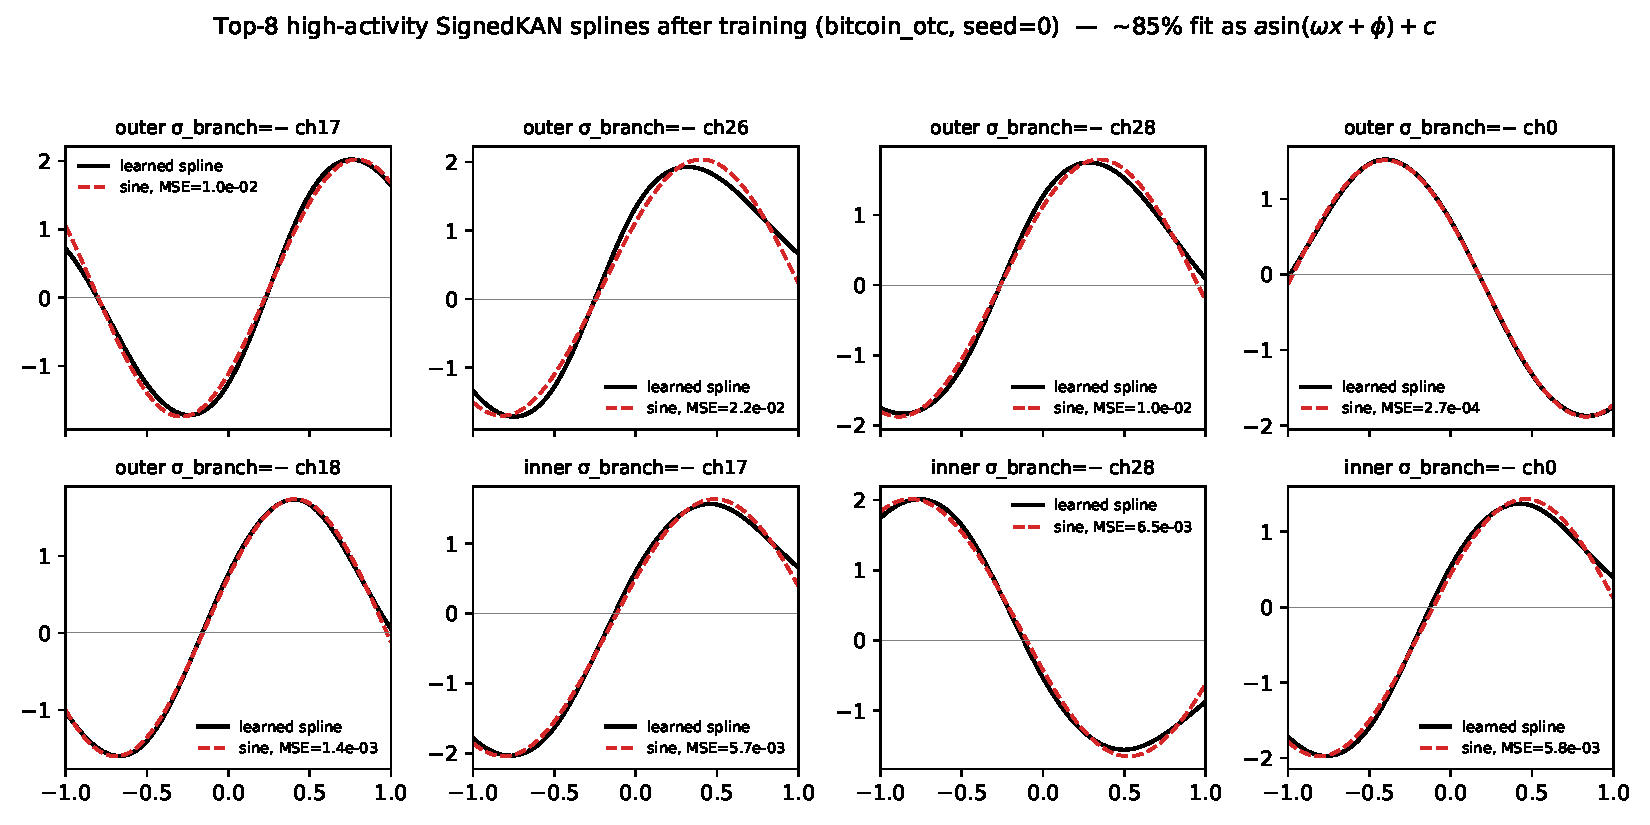
\includegraphics[width=\columnwidth]{figures/sinusoid_distillation.pdf}
\caption{Top-8 high-activity SignedKAN splines on Bitcoin OTC after
$100$-epoch training at the EC recipe. Black: learned spline
output sampled on $[-1, 1]$. Red dashed: best-fitting symbolic form
from the library, all eight here distilling as
$a\sin(\omega x + \phi) + c$. The Fourier-like decomposition emerges
from training, not from architectural prescription.}
\label{fig:sinusoid-distillation}
\end{figure}

Across $128$ splines per (basis, dataset, seed) and $3$ seeds, the
overwhelmingly dominant fitted form is sinusoidal. The
basis-invariance is the load-bearing observation: the model learns
the \emph{shape} of the activation, not the basis-specific
representation. We interpret this as evidence that signed-graph
balance has a low-rank, sinusoidal structure that any sufficiently
flexible basis discovers when fed the Cartwright--Harary triad
incidence.
Figure~\ref{fig:sinusoid-distillation} shows the eight most-active
splines on Bitcoin OTC, with the $a\sin(\omega x + \phi) + c$ fit
overlaid; the residual MSEs are uniformly $<\!10^{-2}$.

\subsection{Heterogeneous skip-connection placement}
\label{sec:heterogeneous-skip}

A complementary architectural axis. The SignedKAN layer has two
spline positions: an inner per-vertex transform and an outer
per-sign-aggregate transform. By analogy with CV networks
(stem--backbone--head), the right composition is rarely
homogeneous --- backbones use skip connections, heads typically do
not. We test six heterogeneous combinations of
$\{\text{none}, \text{residual}, \text{highway}\}$ on
(\textit{inner}, \textit{outer}); the homogeneous-skip-everywhere
baseline is neutral or slightly negative across both fixtures, and
in particular fails on Bitcoin Alpha by $-0.03$ AUC. Heterogeneous
placement reverses this on Bitcoin OTC: every cell is at least
neutral, and the configuration (\textit{inner}: residual,
\textit{outer}: none) reaches $\mathrm{AUC}\!=\!0.8733$
(\,$+0.0033$ over EC, with \emph{zero} added parameters). On the
smaller Alpha fixture, every configuration still pays an AUC cost
(the fixture is too small to absorb the additional gating capacity)
but the macro-$F_1$ gain is consistent across cells
($+0.009$ to $+0.029$), and (\textit{inner}: highway,
\textit{outer}: none) gives $\mathrm{F}_1\!=\!0.7269$
($+0.029$ over EC).

This says something architecturally specific: \textbf{the
``backbone'' of SignedKAN is the inner per-vertex spline}, and that
position benefits from a residual skip; the per-sign-aggregate
outer is closer in role to a classifier head and prefers to stay
unskipped. Adding gating to both positions costs more than placing
it in the right one.

\subsection{Cost--capacity summary}
\label{sec:cost-capacity}

A trained SignedKAN under the EC recipe at $h\!=\!32$ has
$121{,}985$ parameters on Bitcoin Alpha and $189{,}121$ on Bitcoin
OTC. The breakdown, however, is what the cost--capacity discussion
turns on: $\sim\!99\%$ of these parameters are the node-embedding
table $\mathbb{R}^{|V|\times h}$, shared with every embedding-based
signed-GNN; the SignedKAN-specific architectural overhead is
$\sim\!930$ parameters --- two pairs of inner+outer batched-spline
coefficient tensors plus the linear classifier --- which accounts
for $\sim\!0.8\%$ of the model on Alpha and $\sim\!0.5\%$ on OTC.
Pruning at $\tau\!=\!1.8$ then retains $\sim\!22\%$ of that
overhead, distillable into roughly $28$ surviving sinusoidal
symbolic activations.

Table~\ref{tab:param-compare} contextualises the architectural
overhead against representative signed-GNN baselines at matched
hidden dimension on Bitcoin Alpha. The estimates draw on each
paper's reported configuration; exact numbers depend on
implementation choices. Two observations: (i) every embedding-based
signed-GNN spends the same node-embedding budget; (ii) SignedKAN's
architectural overhead is comparable to or smaller than SiNE's MLP
head, smaller than SGCN's two layers of four weight matrices each
(\,$\sim\!8$k overhead), and considerably smaller than SDGNN's
multi-task signed convolution stack.

\begin{table}[t]
\centering
\caption{Parameter-count comparison at $h\!=\!32$ on Bitcoin Alpha
($|V|\!=\!3{,}783$). Architectural overhead is the model size
\emph{minus} the node-embedding table. SignedKAN numbers are
measured; baselines are estimated from their reported architectures
(order-of-magnitude only).}
\label{tab:param-compare}
\setlength{\tabcolsep}{4pt}
\small
\begin{tabular}{@{}lrrr@{}}
\toprule
model & node embed & arch overhead & total \\
\midrule
\textbf{SignedKAN} (ours, EC) & $121{,}056$ & $\mathbf{929}$       & $\mathbf{121{,}985}$ \\
SignedKAN, pruned $\tau\!=\!1.8$ & $121{,}056$ & $\mathbf{\sim\!200}$ & $\mathbf{\sim\!121{,}256}$ \\
SiNE~\cite{wang2017sine}  & $121{,}056$ & $\sim\!2$--$3$k       & $\sim\!123$k \\
SGCN~\cite{derr2018sgcn}  & $121{,}056$ & $\sim\!8$k            & $\sim\!130$--$135$k \\
SDGNN~2021                 & $121{,}056$ & $\sim\!20$--$60$k     & $\sim\!140$--$180$k \\
DSHGNN~2025                & $121{,}056$ & $\sim\!10$--$40$k     & $\sim\!130$--$160$k \\
\bottomrule
\end{tabular}
\end{table}

The pruning compression story is therefore architecturally specific
rather than total-model: the spline overhead drops by $\sim\!4\times$
under threshold-pruning, while the node-embedding table is
unchanged. Total-model compression would require an orthogonal
intervention on the embedding table (product quantisation,
top-$k$ filtering, quantisation-aware training); these are deferred
to a journal extension.

Wall-clock training is $\sim\!13$~s per fit on Bitcoin Alpha and
$\sim\!20$~s per fit on Bitcoin OTC at $200$ epochs with early
stopping on a single mid-range GPU, replicable on a laptop.
Substituting Catmull--Rom for B-spline drops per-iter cost by an
additional $\sim\!2.5\times$ at essentially the same accuracy
(Section~\ref{sec:gap}, Table~\ref{tab:gap}). The combined
fast/sparse/interpretable architecture is the WiP-track contribution
that engineered signed-GNN baselines do not match.